\documentclass[11pt,titlepage]{article}

%Laenderspezifische Einstellungen bzgl. Rechtschreibung, Sonderzeichen und Kodierung
\usepackage[utf8]{inputenc}
\usepackage[english]{babel}
\usepackage[T1]{fontenc}
\usepackage{titlesec}
\usepackage{graphicx}
%\usepackage{subcaption}

\usepackage{mathtools}
\usepackage[thinc]{esdiff}

\usepackage{listings}
\usepackage{color}
\usepackage{courier}
\definecolor{light-gray}{gray}{0.85}
\definecolor{dark-green}{rgb}{0.05,0.65,0.3}
\lstset{
	language=C++,
	numbers=left,
	breaklines=true,
	backgroundcolor=\color{light-gray},
	tabsize=2,
	basicstyle=\footnotesize\ttfamily,
	frame=single,
	inputencoding=utf8,
	extendedchars=true,
	showstringspaces=false,
	commentstyle=\color{dark-green}\ttfamily,
	literate =
	{ä}{{\"a}}1
	{ö}{{\"o}}1
	{ü}{{\"u}}1
	{Ä}{{\"A}}1
	{Ö}{{\"O}}1
	{Ü}{{\"U}}1
	{ß}{{\ss}}1
	{ₙ}{{$_n$}}1
}

\def\ContinueLineNumber{\lstset{firstnumber=last}}
\def\StartLineAt#1{\lstset{firstnumber=#1}}

\usepackage[
a4paper,
top = 2cm,
bottom = 2 cm,
left = 2cm,
right = 2cm,
headheight = 15pt,
includeheadfoot
]{geometry}
\usepackage{fancyhdr}
\usepackage{amssymb}
\usepackage{amsmath}
\usepackage[english]{varioref}
\usepackage{hyperref}

\usepackage{float}
\usepackage{amsthm}

\usepackage{float}

\fancypagestyle{fancy}{
	\fancyhead[R]{Seite \thepage}
	\fancyhead[L]{\leftmark}
	\renewcommand{\headrulewidth}{1.25pt}
	
	\fancyfoot[L]{\tiny{\textit{}}}
	\fancyfoot[R]{\tiny{ Felix Dreßler (k12105003)}}
	\cfoot{}
	\renewcommand{\footrulewidth}{1.25pt}
}

\setlength{\headsep}{10mm}
\setlength{\footskip}{10mm}

\setlength{\parindent}{0mm}
\setlength{\parskip}{1.1ex plus0.25ex minus0.25ex}
\setlength{\tabcolsep}{0.2cm} % for the horizontal padding

\pagestyle{fancy}

\title{Circuit Modelling}
\author{Felix Dreßler (k12105003)\\ email \href{mailto:FelixDressler01@gmail.com}{FelixDressler01@gmail.com}}
\date{\today} %Erstellungsdatum

\renewcommand{\labelenumi}{\roman{enumi})}

\newtheorem{definition}{Definition}
\newtheorem{theorem}{Theorem}
\newtheorem{lemma}{Lemma}

\begin{document}
	\maketitle
	\section{Introduction}
		This chapter should include information about what circuit modelling wants to achieve as well as giving an overview of what this bachelor-thesis is about.
		
		What is this thesis about? \newline
			Modelling and numerically solving systems that arrise from electrical circuits with RLC elements. Furthermore it will briefly discuss on expanding this baseline with more complicated electrical components.
		What is the goal of this thesis?\newline
			The goal of this thesis is to give insight into industrial standards concerning circuit modelling. It aims to elaborate on the underlying concepts of MNA as well as on the most commonly used numerical methods.
		
	\newpage	
	\section{Formulating a Mathematical Model}
	based on DAE lecture and modelling and discretiztation of elec circuit problems.
		\subsection{Network Topology}
			An electrical circuit is usually considered as a graph $(N,E)$ where $N = (n_0, n_1, n_2, ...)$ are the Nodes and $E = (e_{ij})_{ij}$ are the edges, where for some $i$ and some $j$ we have that $e_{ij} = (n_j, n_k)$ is the edge from node $j$ to node $k$. %rewrite that
			We can store this information in an \emph{incidence matrix} $\tilde{A} = (\tilde{a}_{ij})_{ij}$ which is defined by
			\begin{displaymath}
				\tilde{a}_{ij} = 
				\begin{cases}
					1 &   \text{edge $j$ starts at node $i$},\\
					-1 &  \text{edge $j$  ends at node $i$},\\
					0 & \text{else}.				
				\end{cases}
			\end{displaymath}
			We call $u = (u_0, u_1, u_2, ...)$ the corresponding potentials to the nodes $N$. The difference of these potentials is the voltage at the associated edge. To fix the absolute values of these potentials we have to set one node to a fixed potential. We will do that by ``grounding'' the node $n_0$, this means we set the potential $u_0 := 0$. This grounding of a node allows us to remove the corresponding row from the incidence matrix to get the \emph{reduced incidence matrix} $A$. The vector $v = (v_{ij})_{ij}$ represents the voltages at the edges. For some $i$ and some $j$ the voltage at edge $ij$ is $v_{ij} = u_i - u_j$.
			
			We will later see, that the components of an electrical crircuit, which will be installed along the edges, describe a relationship between the edges current and its voltage. Thus a current vector $i = (i_1, i_2, i_3, ...)$ containing the currents along the edges is required.
			
		\subsection{Energy Conservation Laws}
			To fully fix all the variables that arrise in the model of an electrical circuit we will need some \emph{conservation laws}:
			\begin{itemize}
				\item \textbf{Kirchhoff's voltage law (KVL):} \newline
					The sum of voltages along each loop of the network must equal to zero. Using the incidence matrix $A$ this law can be formulated as
					\begin{equation}
						\label{KVL}
						A^\top * u = v.
					\end{equation}
				\item \textbf{Kirchhoff's current law (KCL):} \newline
					For any node, the sum of currents flowing into the node is equal to the sum of currents flowing out of the node. Using the incidence matrix $A$ again, this law can be formulated as
					\begin{equation}
						\label{KCL}
						A * i = 0.
					\end{equation}
			\end{itemize}
		
		\subsection{Electrical Components and their relations}
			Electrical components are described by equations relating their edge voltage $v$ to their edge current $i$.
			\begin{itemize}
				\item \textbf{Resistor} \newline
					$v = R*i$ or $i = G*u$
					\begin{figure}[H]
						\centering
						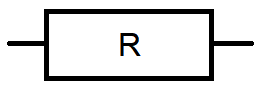
\includegraphics[width=2cm]{pictures/resistor.png}
					\end{figure}
				\item \textbf{Capacitor} \newline
					$Q = C * v$ → $I = C*\dot{v}$
					\begin{figure}[H]
						\centering
						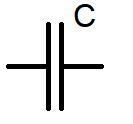
\includegraphics[width=2cm]{pictures/capacitor.png}
					\end{figure}
				\item \textbf{Coil} \newline
					$\Phi = L*i$ → $v = L*\dot{i}$
					\begin{figure}[H]
						\centering
						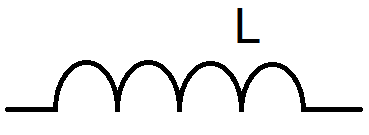
\includegraphics[width=3cm]{pictures/coil.png}
					\end{figure}
				\item \textbf{Voltage Source} \newline
					$v = v_{src}$
					\begin{figure}[H]
						\centering
						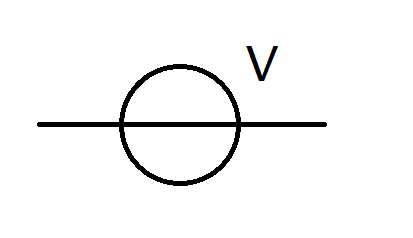
\includegraphics[width=4cm]{pictures/voltage_source.png}
					\end{figure}
				\item \textbf{Current Source} \newline
					$i = i_{src}$
					\begin{figure}[H]
						\centering
						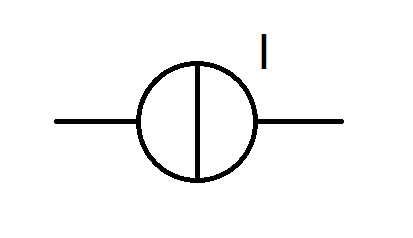
\includegraphics[width=4cm]{pictures/current_source.png}
					\end{figure}
				\item Diode - to be filled with information after the rest is complete
				\item Transistor
			\end{itemize}
		
		\subsection{Modified Nodal Analysis - MNA}
			
			num gew dgl steif n steif - seite 422 \newline
			modelling discr circ prob - seite 19
			
			To analyse the network further we will sort the reduced incidence matrix $A$ such that is has the block form
			\begin{displaymath}
				A = (A_R A_C A_L A_V A_I)
			\end{displaymath}
			where $A_R$, $A_C$, $A_L$, $A_V$ and $A_I$ all include the collumns that are related to the resistors, capacitors, coils, voltage sources and current sources. 
			
			To mathematically describe the circuit we will use \emph{modified nodal analysis} (or short MNA). MNA uses the node voltages as well as the currents of the coils and the voltage sources as unknowns and is based on the conservation laws
			\begin{equation}
				\label{KCL}
				Ai(t) = 0 
			\end{equation}
			\begin{equation}
				\label{KVL}
				v = A^\top u(t)
			\end{equation}
			
			as well as on the voltage-current relations of the electrical components. By replacing all edge-currents with their respective voltage-current relation and ell egde-voltages with their node-potentials we obtain the MNA-equations
					
			\begin{displaymath}
				\begin{aligned}
					A_C C A_C^\top \dot{u} + A_R G A_R^\top u + A_L i_L + A_V i_V + A_I i_{src} &= 0 \\
					L \dot{i_L}	- A_L^\top u &= 0 \\
					-A_V^\top + v_{src} &= 0.
				\end{aligned}	
			\end{displaymath}
			In matrix form these read as
			\begin{displaymath}
				\begin{pmatrix}
					A_C C A_C^\top & 0 & 0 \\
					0 & L & 0 \\
					0 & 0 & 0
				\end{pmatrix}
				*
				\begin{pmatrix}
					\dot{u} \\
					\dot{i_L} \\
					\dot{i_V}
				\end{pmatrix}
				+
				\begin{pmatrix}
					A_R G A_R^\top & A_L & A_V \\
					-A_L^\top & 0 & 0 \\
					-A_V^\top & 0 & 0 
				\end{pmatrix}
				*
				\begin{pmatrix}
					u \\
					i_L \\
					i_V
				\end{pmatrix}
				=
				\begin{pmatrix}
					-A_I i_{src} \\
					0 \\
					-v_{src}
				\end{pmatrix} , 
			\end{displaymath}
			where the diagonal matrices $C$, $G$ and $L$ contain the capacities, conductivities and inductivities.
		
		\subsection{Energy \textbf{bilanz??????????}}
		
		\subsection{Charge/Flux oriented formulation of MNA}
			Again using KCL \ref{KCL} and the component equations we formulate a system of equations. (\textbf{more here}) What is flux and charge - explain either here or witht the components
			
			\begin{align}
				A_C\dot{q} + A_R r(A_R^\top u,t) + A_L i_L + A_V i_V + A_I i(A^\top u, \dot{q}, i_L, i_V, t) &= 0 \label{charge/flux-1} \\
				\dot{\phi} - A_L^\top u &= 0 \label{charge/flux-2} \\
				v(A^\top u, \dot{q}, i_L, i_V, t) - A_V^\top u &= 0 \label{charge/flux-3} \\
				q - q_C(A_C^\top u) &= 0 \label{charge/flux-4} \\
				\phi - \phi_L(i_L) &= 0  \label{charge/flux-5} 
			\end{align}
			
			Using
			\begin{description}
				\item node potentials $u$,
				\item branch currents through voltage and flux controlled elements $i_V$ and $i_L$,
				\item charges and fluxes $q$ and $\phi$,
				\item voltage dependent resistors $r$,
				\item voltage and current dependent charge and flux sources $q_C$ and $\phi_L$,
				\item controlled current and voltage sources $i_src$ and $v_src$.
			\end{description} 
			
			\begin{figure}[H]
				\centering
				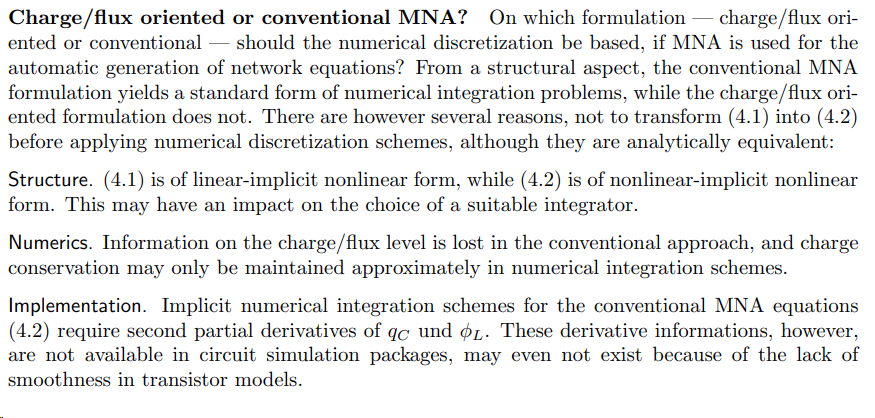
\includegraphics[width=0.7\linewidth]{screenshot007}
				\caption{}
				\label{fig:screenshot007}
			\end{figure}
			
		
	\newpage	
	\section{Differential Algebraic Equations}
	
		von num gew dgl niochtsteife steife und dae
	
		\subsection{Abstract Problem}
			\begin{equation}
				\label{Abstract_DAE}
				F(t, y(t), y'(t)) = 0 \qquad \forall t \in I
			\end{equation}
			
			with $F:\mathbb{R} \times \mathbb{R}^N \times \mathbb{R}^N \to \mathbb{R}^N$ sufficiently smooth. We will focus on linear time invaraiant systems of the form
			
			\begin{displaymath}
				E u'(t) = A u(t) + f(t).
			\end{displaymath}
			
			With $E, A \in \mathbb{R}^{n \times n}$. If $E$ is regular, then this system is just an ordinary differential equation, thus we assume $E$ to be singular to obtain a ``true'' DAE. 
			
			In the following chapters we will discuss important analytical properties of this such sytems. We will discuss the solvability and the index of these systems.
			
		\subsection{Types of DAEs}
		
			\begin{itemize}
				\item \textbf{Linear systems with constant coeffiecients} \newline
					are systems of the form 
					\begin{equation}
						\label{DAE-const-coeff}
						A y'(t) + B y(t) = f(t)
					\end{equation}
					with $A,B \in \mathbb{R}^{n \times n}$, $A$ singular and $f(t)$ a function.
				\item \textbf{linear time dependent systems} \newline
					\begin{displaymath}
						A(t) y'(t) + B(t) y(t) = f(t)
					\end{displaymath}
					with $A(t),B(t),f(t)$ functions.
				\item  \textbf{structured (non-linear) systems} \newline
					are semi-explicit systems of the form
					\begin{displaymath}
						y'(t) = f(t, y(t), z(t)),
						0 = g(t,y(t),z(t))
					\end{displaymath}
					with $f$ and $g$ functions.
			\end{itemize}
			
			For our analysis of electrical networks we will focus on linear systems with constant coefficients. (where do the other systems arrise? what are they about?)
			
			\subsubsection{Weierstraß-Kronecker Normalform}
				kapitel aus buch seite 399 num gew dgl steif, kapitel 13.2.2
			
				To determine the solvability of a linear system with constant coefficients \ref{DAE-const-coeff} we first need to introduce a Normalform for the system, the \emph{Weierstraß-Kronecker Normalform}. This Normalform is dependant on the family $\{A,B\} := \{ \mu A+B|\mu \in \mathbb{R} \}$, which is called the  \emph{matrix pencil} of the DAE.
				
				\begin{definition}
					The matrix pencil $\{ A,B\}$ is called \emph{regular} if there exists some $c \in \mathbb{R}$, such that $(cA+B)$ is regular ($det(cA+B) \neq 0$), otherwise it is called singular.
				\end{definition}
			
				\begin{theorem}[Jordan Normalform]
					For every matrix $Q \in \mathbb{R^{n \times n}}$ there exists a regular matrix $T \in \mathbb{C}^{n \times n}$, such that
					\begin{displaymath}
						T^{-1}QT = J = diag(J_1, ..., J_r) \quad \text{with} \quad J_i = 
						\left(
						\begin{matrix}
							\lambda_i & 1 & & 0 \\
							0 & \lambda_i & \ddots & \vdots \\
							& \ddots & \ddots & 1 \\
							0 & \hdots & 0 & \lambda_i
						\end{matrix}
						\right)
						\in \mathbb{C}^{m_i \times m_i}
					\end{displaymath} 
					and $n = m_1 + ... + m_r$.
				\end{theorem}
				quote that from somewhere.
				
				translate that:
				
				The matrix $J$ is called Jordan Normalform of $Q$, the $J_i$ are called Jordan Blocks, where $\lambda_i$ are the eigenvalues of $Q$. The matrix $J$ is uniquely determined by $Q$ except for the arrangement of the diagonal blocks. If $Q$ posesses only real eigenvalues, then $T$ can also be choosen from the reals. \newline
				A transformation from $A$ and $B$ in \ref{DAE-const-coeff} enables a seperation into differential and algebraic variables.	
				
				aus buch seite 401
				\begin{theorem}
					\label{Kronecker-Normalform}
					Let $\{ A,B \}$ be a regular matrix pencil. There exist $P,Q \in \mathbb{C}^{n \times n}$ such that
					\begin{displaymath}
						PAQ = 
						\left(
						\begin{matrix}
							I_d & 0 \\
							0 & N 
						\end{matrix}
						\right), \quad
						PBQ = 
						\left(
						\begin{matrix}
							R & 0 \\
							0 & I_{n-d}
						\end{matrix}
						\right)
					\end{displaymath}
					where
					\begin{displaymath}
						N = diag(N_1, ..., N_r) \quad \text{with} \quad N_i = 
						\left(
						\begin{matrix}
							0 & 1 & & 0\\
							& \ddots &\ddots & \\
							& & & 0 & 1 \\
							0 & & & 0
						\end{matrix}
						\right)
						\in \mathbb{R}^{n_i \times n_i}
					\end{displaymath}
					and R has Jordan Normalform.
				\end{theorem}
				\begin{proof}
					Becuase $\{A,B\}$ is a regular matrix pencil, there exists $c \in \mathbb{R}$ such that $(cA+B)$ is regular. Set
					\begin{displaymath}
						\hat{A} := (cA+B)^{-1}A, \quad \hat{B} := (cA+B)^{-1}B.
					\end{displaymath}
					Considering 
					\begin{displaymath}
						(cA+B)^{-1}(cA+B) = I \implies (cA+B)^{-1}B+c(cA+B)^{-1}A = I ,
					\end{displaymath}
					we get that
					\begin{displaymath}
						\hat{B} = I-c \hat{A} .
					\end{displaymath}
					Let $J_ {\hat{A}}$ be the Jordan Normalform of $\hat{A}$, this means that there exists a regular matrix $T_1$ such that
					\begin{displaymath}
						T_1^{-1}AT_1 = J_{\hat{A}} =
						\left(
						\begin{matrix}
							W & 0 \\
							0 & \tilde{N} 
						\end{matrix}
						\right) .
					\end{displaymath}
					The matrix $W$ contains the Jordanblocks with Eigenvalues which are nonzero, the matrix $\tilde{N}$ contains the Jordan blocks with Eigenvalues equal to zero, thus $\tilde{N}$ is \emph{nilpotent}.
					The Jordan Normalform $J_{\hat{B}}$ of $\hat{B}$ is given by
					\begin{displaymath}
						T_1^{-1} \hat{B} T_1 = J_{\hat{B}} = 
						\left(
						\begin{matrix}
							I-cW & 0 \\
							0 & I-c\tilde{N}
						\end{matrix}
						\right) .
					\end{displaymath}
					The following two transformations will allow us to get the desired structure.
					First we will transform $J_{\hat{A}}$ with
					\begin{displaymath}
						T_2 :=
						\left(
						\begin{matrix}
							W & 0 \\
							0 & I-c\tilde{N}
						\end{matrix}
						\right)
					\end{displaymath}
					in
					\begin{displaymath}
						T_2^{-1}J_{\hat{A}} = 
						\left(
						\begin{matrix}
							I & 0 \\
							0 & (I-c\tilde{N})^{-1}\tilde{N}
						\end{matrix}
						\right)
					\end{displaymath}
					and $J_{\hat{B}}$ in
					\begin{displaymath}
						T_2^{-1}J_{\hat{B}} =
						\left(
						\begin{matrix}
							W^{-1}-cI & 0 \\
							0 & I
						\end{matrix}
						\right) .
					\end{displaymath}
					Let now $R$ be the Jordan Normalform of $(W^{-1}-cI)$ and $N$ be the Normalform of $(I-c\tilde{N})^{-1}\tilde{N}$, this means
					\begin{displaymath}
						T_W^{-1}(W^{-1}-cI)T_W = R \quad \text{and} \quad T_{\tilde{N}}^{-1}(I-c\tilde{N})^{-1}\tilde{N}T_{\tilde{N}} = N
					\end{displaymath}
					Considering
					
					\begin{figure}[H]
						\centering
						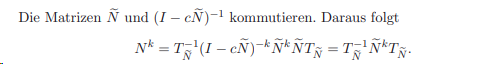
\includegraphics[width=0.7\linewidth]{screenshot001}
						\caption{fig 1, i dont get why}
						\label{fig:screenshot001}
					\end{figure}
					
					
					The nilpotent matrix $N$ thus has the nilpotency index $k$. A transformation with
					\begin{displaymath}
						T_3 := 
						\left(
						\begin{matrix}
							T_W & 0 \\
							0 & T_{\tilde{N}}
						\end{matrix}
						\right)
					\end{displaymath}
					transforms $T_2^{-1}J_{\hat{A}}$ into the Jordan Normalform
					\begin{displaymath}
						J_{\tilde{A}} := T_3^{-1}T_2^{-1}J_{\hat{A}}T_3 = T_3^{-1}T_2^{-1}T_1^{-1}\hat{A}T_1T_3 = 
						\left(
						\begin{matrix}
							I & 0 \\
							0 & N
						\end{matrix}
						\right)
					\end{displaymath}
					and $T_2^{-1}J_{\hat{B}}$ into
					\begin{displaymath}
						J_{\tilde{B}} := T_3^{-1}T_2^{-1}J_{\hat{B}}T_3 = T_3^{-1}T_2^{-1}T_1^{-1}\hat{B}T_1T_3 = 
						\left(
						\begin{matrix}
							R & 0 \\
							0 & I
						\end{matrix}
						\right) .
					\end{displaymath}
					Now set
					\begin{displaymath}
						P:= T_3^{-1}T_2^{-1}T_1^{-1}(cA+B)^{-1} \quad \text{and} \quad Q = T_1T_3
					\end{displaymath}
					to get the statement.
				\end{proof}
				
				\begin{definition}
					The nilpotency index $k$ from the Weierstraß-Kronecker Normalform of a matrix pencil $\{A,B\}$ with $A$ singular is called the \emph{Kronecker-Index} of $\{A,B\}$. We write $ind\{A,B\}$. For $A$ regular we set $ind\{A,B\} = 0$.
				\end{definition}
				
				next lemma needs quotation, it is lemma 13.2.1
				
				\begin{lemma}
					The Kronecker-Index $ind\{A,B\}$ is independant of the choice of the matrices $P$ and $Q$.
				\end{lemma}
				
				\begin{figure}
					\centering
					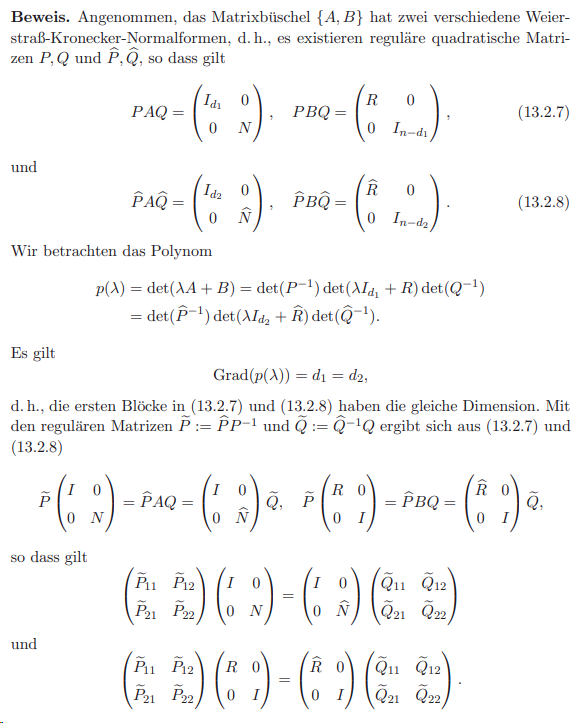
\includegraphics[width=0.7\linewidth]{screenshot003}
					\caption{}
					\label{fig:screenshot003}
				\end{figure}
				
				\begin{figure}
					\centering
					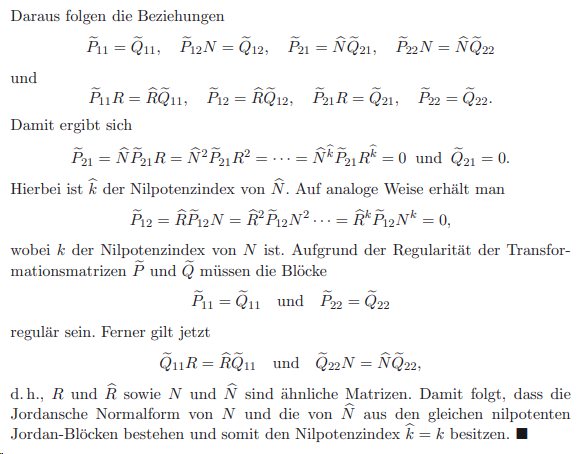
\includegraphics[width=0.7\linewidth]{screenshot004}
					\caption{}
					\label{fig:screenshot004}
				\end{figure}
				
				
				Lemma 13.2.2 maybe
				
				Using the findings above we are able to Transform the initial DAE \ref{DAE-const-coeff} using the matrix $P$ from \ref{Kronecker-Normalform}. By multiplying $P$ from the left we obtain
				
				\begin{displaymath}
					P A y'(t) + P B y(t) = P f(t) .
				\end{displaymath}
			
				Setting
				
				\begin{displaymath}
					y = Q
					\left(
					\begin{matrix}
						u \\
						v
					\end{matrix}  
					\right) 
					, \quad
					Pf(t) = 
					\left(
					\begin{matrix}
						s(t) \\
						q(t)
					\end{matrix}
					\right)
					\quad \text{with} \quad
					u,s \in \mathbb{R}^d ,
				\end{displaymath}
				
				we get a system of the form
				
				\begin{equation}
					\label{transformed-DAE-const-coeff}
					\begin{aligned}
						u'(t) + Ru(t) &= s(t) \\
						Nv'(t) + v(t) &= q(t)
					\end{aligned}
				\end{equation}
				
				The first equation is an ordinary differential equation of first order and posesses a unique solution $u(t)$ in $[t_0,t_l]$ for any starting values $u_0 \in \mathbb{R}^d$. Additionally setting $q(t) \in C^{k-1}([t_0,t_l])$ then differentiating the second equation in \ref{transformed-DAE-const-coeff} gives (\textbf{whyyyyyyy??????})
				
				\begin{displaymath}
					\begin{aligned}
						v(t) &= q(t) - Nv'(t) = q(t) - N(q(t)-Nv'(t))' = q-Nq'+N^2v'' \\
						&= q-Nq'+N^2(q-Nv')'' = q-Nq'+N^2q''-N^3v''' \\
						&\vdots \\
						&= q-Nq'+...+(-1)^{k-1}N^{k-1}q^{(k-1)}+(-1) \underbrace{N^kv^{(k)}}_{=0}
					\end{aligned}
				\end{displaymath}
				\begin{equation}
					\label{solution-to-transformed-DAE-const-coeff-part2}
					= \sum_{i=0}^{k-1} (-1)^iN^iq^{(i)}(t) 
				\end{equation}
				where $k$ is the nilpotency index of $N$. This expression gives an explicit solution for $v(t)$ in $[t_0,t_l]$ with $v(t) \in \mathbb{R}^{d-1}$. It shows the depencdency of the solution and its derivatives. The higher the Kronecker index $k$ gets, the more differentiations of $q(t)$ have to be performed.

				The Kronecker index $k$ shows, that $k$ differentiations are required to receive an ordinary differential equation.
		\subsection{Index of a Differential Algebraic Equation}
		
			The Index of a DAE gives us insight about it's numerical properties and in general about the solvability. In general, the higher the index, the harder it is, to solve the system. 
			
			We will consider two types of index concepts, the differentiation index and the perturbation index.
					
			\begin{definition}[differentiation index]
				Consider the differential algebraic equation \ref{Abstract_DAE} to be uniquely locally solvable and $F$ suffieciently smooth differentiable. For a given $m \in \mathbb{N}$ consider
				\begin{displaymath}
					\begin{aligned}
						F(t,y,y') &= 0, \\
						\diff{F(t,y,y')}{t} &= 0, \\
						&\vdotswithin{=} \\
						\diff[m]{F(t,y,y')}{t} &= 0.
					\end{aligned}
				\end{displaymath}
				The smallest natural number $m$ for which the above System results in an explicit system of the form
				\begin{displaymath}
					y' = \phi(t,y)
				\end{displaymath}
				from which $y$ can be determined is called \textbf{differentiation index}.
			\end{definition}
			
			In the previous chapter we have already discussed, that for a DAE with constant coefficients \ref{DAE-const-coeff} and a regular matrix pencil $\{A,B\}$  we need $k = ind\{A,B\}$ differentiations to receive an ordinary differential equation. This means that the Kronecker index $k$ is equal to the differentiation index in the case of a DAE with constant coefficients.
			
			\begin{definition}[perturbation index]
				Let $y(t)$ be the exact solution to \ref{Abstract_DAE}. This problem has the \textbf{perturbation index} $k \in \mathbb{N}$ along $y(t), t_0 \leq t \leq T$ if for all  $\tilde{y}(t)$ with $F(t, \tilde{y}, \tilde{y}') = \delta(t)$ the inequality
				\begin{displaymath}
					||y(t)-\tilde{y}(t)|| \leq C \left(||y(t_0)-\tilde{y}(t_0)||+\sum_{j=0}^{k}\max_{t_0 \leq \xi \leq T} \left\rVert 		\int_{t_0}^{\xi}\diff[j]{\delta}{\tau}(\tau)d \tau \right\rVert \right)
				\end{displaymath}
				for the smallest number $k$.
			\end{definition}	
	
			for lin const nilpot ind  = ind + proof
			
			\begin{figure}[H]
				\centering
				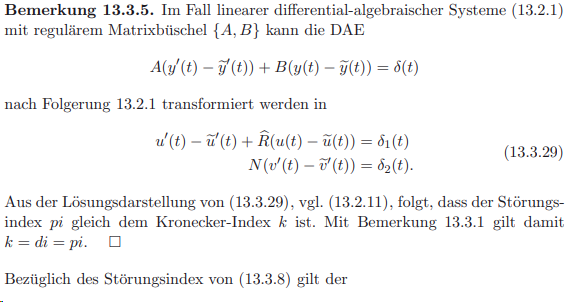
\includegraphics[width=0.7\linewidth]{screenshot005}
				\caption{}
				\label{fig:screenshot005}
			\end{figure}
			
		
		
	\newpage
	\section{Index Analysis of the MNA}
		
		der ane satz do + proof hopefully
		
		seite 22 kap 7 netw top and dae ind for rlc - modelling and discretization circ prob
		
		In the linear case, the capacitances, inductances and resistances are symmetrical positive definite (We consider them as matrices in this case). In the nonlinear case ... . Then it is called an RLC network.
		
		In our further analysis we will only consider such RLC networks.
		
		\subsection{General Index analysis}
		
			Assuming the system only contains linear elements or is linearized at an operating point in order to investigate the system behaviour then the corresponding network equation represent a DAE with constant coefficients \ref{DAE-const-coeff}. Ww will denote $x=(u i_L i_V)^\top$.
			
			\begin{itemize}
				\item \textbf{ODE-case}: \newline
					The matrix $B$ is regular in \ref{DAE-const-coeff}. This is the case if
					\begin{figure}[H]
						\centering
						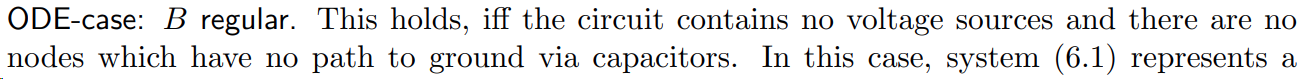
\includegraphics[width=0.7\linewidth]{screenshot006}
						\caption{}
						\label{fig:screenshot006}
					\end{figure}
					, then the system represents  alinear-implicit system of ODEs and can be transformed into the explicit ODE sytstem
					\begin{displaymath}
						\dot{x}=B^{-1}(-Ax+f(t))
					\end{displaymath}
					
				\item \textbf{DAE-case}:
					The matrix $B$ is singular in \ref{DAE-const-coeff}. In the following we will assume $D$ to be regular. Multiplying with $D^{-1}$ from the left side produces
					\newline
					nevermind thats the same as we did in the \ref{DAE-const-coeff} chapter. - reference to that an explain in these terms. - page 20
			\end{itemize}
		
		\subsection{Topological Conditions}
			For this we consider RLC networks with independant voltage and current sources (\textbf{what does that mean?}). To obtain the perturbation index of the MNA we perturb the right-hand side of  
			\newline reference to Tischendorf
		
		
	\newpage
	\section{Numerical Solutions}
		This chapter focuses on the numerical solution of the mentioned systems. (based on the DAE-lecture)
		It will include Code that illustrates some of the shown procedures.
		
		We will first focus on the general methods used for solving a more general problem
		\begin{equation}
			\label{general numerical problem}
			\begin{align}
				y'(t) &= f(t,y), \quad t \in [t_0, t_l], \\
				y(t_0) &= y_0.
			\end{align}
		\end{equation}
		
		We will presume that the function $f(t,y)$ is continuous 
		
		
		from book circuit modelling 35-47
		
		\subsection{Single-Step-Methods}
			page 46 modelling circuit
			
			page 20 num gew dgl
		\subsection{Multistep-Methods}
			based on chapter 4 of book num gew dgl steif nichtsteif \newline
			Linear multistep methods use approxiamtions $u_{m+l}$ along the gridpoints $t_{m+l}, \quad l=0,1,...,k-1$ to calculate the new approximation $u_{m+k}$ at $t_{m+k}$. WE will first discuss topics related to the order of the methods depending on its parameters, stability and convergence.
			
			\begin{definition}
				For given $\alpha_0, ..., \alpha_k$ and $\beta_0, ..., \beta_k$ the iteration rule
				\begin{equation}
					\label{linear-multistep-method}
					\sum_{l=0}^{k} \alpha_l u_{m+l} = h \sum_{l=0}^{k} \beta_l f(t_{m+l}, u_{m+l}), \quad m=0,1,...,N-k
				\end{equation}
				is called a \emph{linear multistep method} (linear k-step method). It is always assumed that $\alpha_k \neq 0$ and $|\alpha_0| + |\beta_k| > 0$. If $\beta_k=0$ holds, then the method is called explicit, otherwise implicit.
			\end{definition}
			
			\begin{figure}[H]
				\centering
				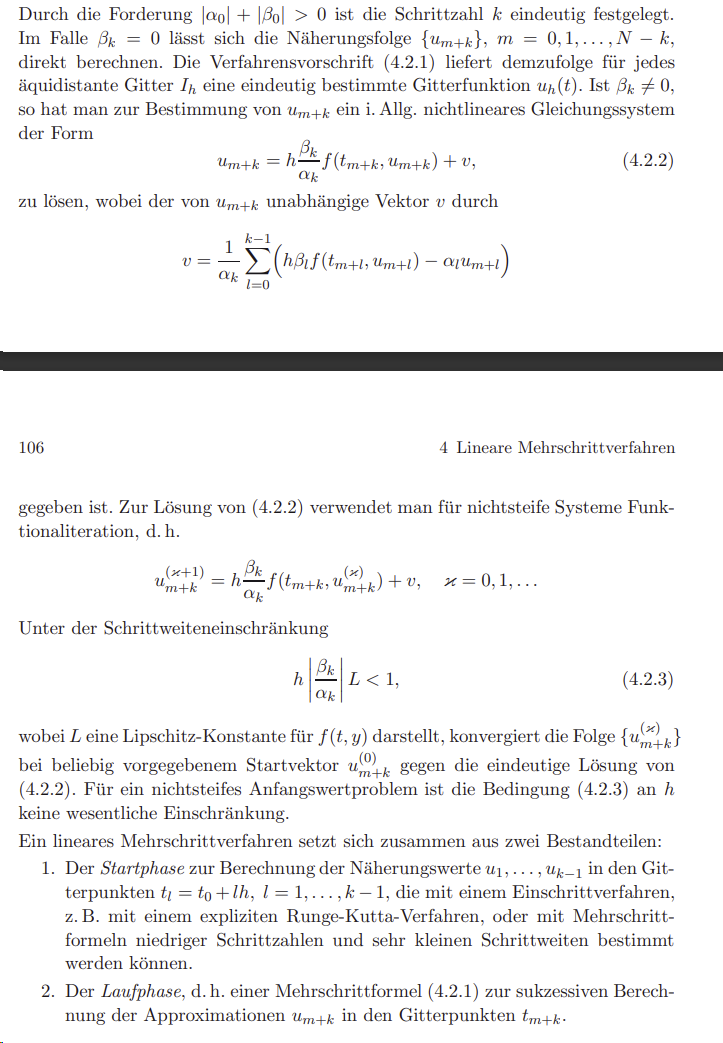
\includegraphics[width=0.7\linewidth]{screenshot010}
				\caption{}
				\label{fig:screenshot010}
			\end{figure}
		
			A linear multi-step method consists of two parts:
			\begin{enumerate}
				\item In the \emph{starting-phase} approximations $u_1,...,u_{k-1}$ for the first $k-1$ gridpoints $t_l = t_0+th, l=1,...,k-1$ are calculated using a single-step method. For example using an explicit Runge-Kutta Methodor a multi-step method with fewer steps.
				
				\item  In the \emph{run-phase} the multi-step formula is used to determine new approximations $u_{m+k}$ for the gridpoint $t_{m+k}$
			\end{enumerate}
			
			For theoretical analysis of the multi-step methods we consider the generating polynomials
			\begin{equation}
				\rho(x) := \sum_{l=0}^{k} \alpha_l x^l
			\end{equation}
			\begin{equation}
				\sigma(x) := \sum_{l=0}^{k} \beta_l x^l
			\end{equation}
		
			\begin{figure}[H]
				\centering
				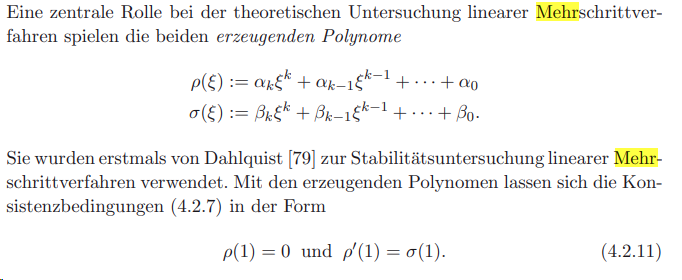
\includegraphics[width=0.7\linewidth]{screenshot013}
				\caption{}
				\label{fig:screenshot013}
			\end{figure}
			
			
			\subsubsection{Consistency and order}
				local discretization error - def 4.2.2
				\begin{definition}
					Let $\tilde{u}_{m+k}$ be the result of one step of the multi-step method \ref{linear-multistep-method} with the start-vectors $u_m, u_{m+1}, ..., u_{m+k-1}$ lying on the exact solution $y(t)$ of the problem \textbf{reference}. This means
					\begin{displaymath}
						\alpha_k \tilde{u}_{m+k} = \sum_{l=0}^{k-1} \left( h \beta_l f(t_{m+l}, y(t_{m+l})) - \alpha_l y(t_{m+l}) \right) + h \beta_k f(t_{m+k}, \tilde{u}_{m+k}) .
					\end{displaymath}
					Then
					\begin{displaymath}
						le_{m+k} = le(t_{m+k}) = y(t_{m+k}) - \tilde{u}_{m+k}, \quad m=0,1,...,N-k
					\end{displaymath}
					 is called the \emph{local discretization error} (local error) of the linear multi-step method \ref{linear-multistep-method} at the point $t_{m+k}$.
				\end{definition}
				
				We will assign the linear difference opreator
				\begin{equation}
					L[y(t),h] = \sum_{l=0}^{k} \left( \alpha_l y(t+lh) - h \beta_l y'(t+lh) \right)
				\end{equation}
				to the local discretization error. Using this we gain the following definition.
			
				\begin{definition}
					A linear multi-step method is called \emph{preconsistent} if for all functions $y(t) \in C^1[t_0,t_l]$
					\begin{displaymath}
						\lim\limits_{h \to 0} L[y(t),h]=0
					\end{displaymath}
					holds. It is called \emph{consistent}, if for all functions $y(t) \in C^2[t_0,t_l]$
					\begin{displaymath}
						\lim\limits_{h \to 0} \frac{1}{h} L[y(t),h] = 0
					\end{displaymath}
					holds. It has the \emph{consistency order p}, if for all functions $y(t) \in C^{p+1}[t_0, t_l]$
					\begin{displaymath}
						L[y(t),h] = \mathcal{O}(h^{p+1}) \quad \text{for} \quad h \to 0
					\end{displaymath}
					holds.
				\end{definition}

				\begin{figure}[H]
					\centering
					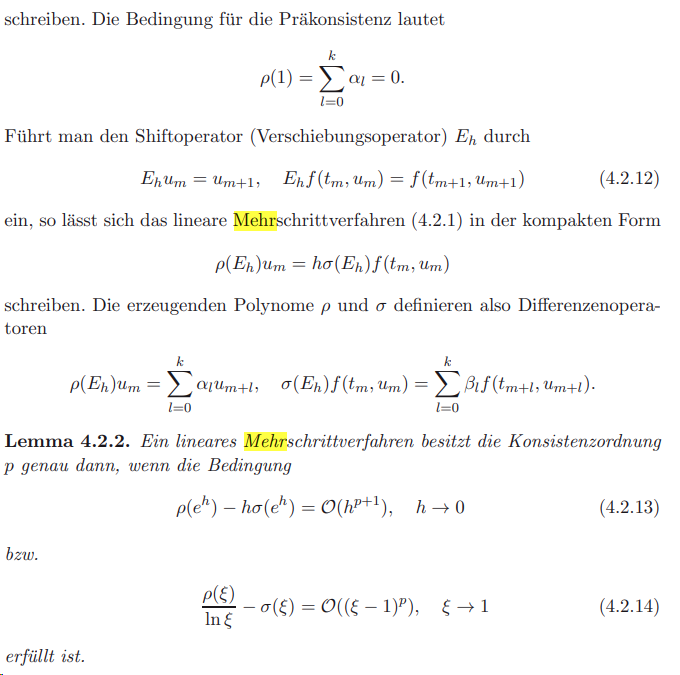
\includegraphics[width=0.7\linewidth]{screenshot014}
					\caption{}
					\label{fig:screenshot014}
				\end{figure}
				

			
			\subsubsection{Convergence and stability}
			
				\begin{definition}
					A linear multi-step method is called \emph{zero-stable} if all solutions of the difference equation
					\begin{displaymath}
						\sum_{l=0}^{k} \alpha_l u_{m+l} = 0
					\end{displaymath}
					are bounded.
				\end{definition}
			
				\begin{theorem}
					A linear multi-step method is zero-stable, if and only if the polynomial $\rho(x)$ fullfills the root-condition, this means:
					\begin{enumerate}
						\item All roots $\bar{x}$ of $\rho(x)$ are within the unit-circle $|\bar{x}| \leq$ in the complex plane.
						\item All roots $\bar{x}$ with $|x| = 1$ are singular.
					\end{enumerate}
				\end{theorem}

		
			\textbf{from circuit book below, above from modelling book}
		
			\subsection{Implicit linear multi-step formulas}
				These kinds of multi-step methods are conventionally used to numerically solve the systems obtained using modified nodal analysis. 
				
				The conventional approach can be split into three main steps:
				\begin{enumerate}
					\item Computation of consistent initial values
					\item numerical integration based on multi-step schemes
					\item transformation of the DAE into a nonlinear system and its numerical solutioon by Newton's procedure (?????????????????will not be discussed further because not very specific)
				\end{enumerate}
			
				\textbf{Consistant initial values} 
				\begin{figure}[H]
					\centering
					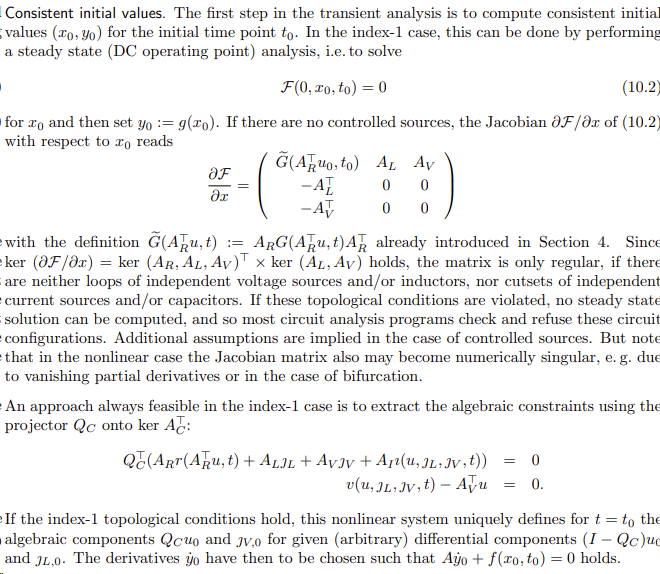
\includegraphics[width=0.7\linewidth]{screenshot009}
					\caption{}
					\label{fig:screenshot009}
				\end{figure}
				
				\textbf{Nunmerical integration}.
				
				
			\subsubsection{BDF schemes and trapezoidal rule}
				
			
			
			
	
\end{document}